% !TEX ecnoding = UTF-8 Unicode

\documentclass[a4paper]{article}

\usepackage{color}
\usepackage{url}
\usepackage[T1]{fontenc}
\usepackage[utf8]{inputenc}
\usepackage{graphicx}
\usepackage{caption}

\graphicspath{ {images/} }
\usepackage{listings}

\usepackage[english,serbian]{babel}

\usepackage[unicode]{hyperref}
\hypersetup{colorlinks, citecolor=green,filecolor=green,linkcolor=blue,urlcolor=blue}

\begin{document}

\title{Naslov\\ \small{Seminarski rad u okviru kursa\\Metodologija stručnog i naučnog rada\\ Matematički fakultet}}

\author{Aleksandra Kovačević, David Ivić, Sreten Kovačević\\ aleksandrakovacevic099@gmail.com, 310ddavi@gmail.com,\\ sretenkvcvc94@gmail.com}
\date{26.~mart 2015.}
\maketitle

\abstract{
}

\tableofcontents

\newpage

\section{Uvod}
\section{Bezbednost veb servera}


Sa pojavom Veb 2.0, pove\'{c}anjem deljenja informacija preko socijalnih mre\v{z}a i kori\v{s}\'{c}enjem veba kao sredstva poslovanja i pru\v{z}anja razli\v{c}itih informacija bezbednost sajtova \v{c}esto biva ugro\v{z}ena direktnim upadima od strane zlonamernih programera.

Zlonamerni programeri(u daljem tekstu hakeri) ili nastoje da kompromituju korporativnu mre\v{z}u ili navode krajnje korisnike koji pristupaju mre\v{z}i ka preuzimanju sadr\v{z}aja \v{c}ijeg rizika nisu svesni (zlonamerni programi-virusi). Kao rezultat toga, industrija obra\'{c}a veliku pa\v{z}nju na bezbednost samih veb aplikacija, pored bezbednosti osnovne ra\v{c}unarske mre\v{z}e i operativnih sistema.

\textbf{Bezbednost veb sajtova} je grana bezbednosti informacija koja se bavi bezbedno\v{s}\'{c}u veb sajtova, veb aplikacija i veb servera. Bezbednost veb aplikacija se oslanja na principe bezbednosti aplikacija uop\v{s}te, ali ih primenjuje specifi\v{c}no za internet i veb sisteme.
Bezbednost veb servera je za\v{s}tita informacija dostupnih preko veb servera. Te informacije se mogu ugroziti pove\'{c}anim sigurnosnim rizicima i propustima prilikom implementacije.


\subsection{Sigurosni rizici}
Najve\'{c}i sigurnosni rizici poti\v{c}u iz nerazumevanja sposobnosti hakera. Kada se razmi\v{s}lja o za\v{s}titi aplikacije, ne sme se voditi mi\v{s}lju: sve \v{s}to je prikazano, biva na\v{s}e ograni\v{c}enje onoga \v{s}to mo\v{z}emo da u\v{c}inimo. Sve \v{s}to predstavlja klijentsku stranu i ograni\v{c}enja koja su na njoj nametnuta se veoma lako mogu zaobi\'{c}i.
\textbf{Pretra\v{z}iva\v{c} ne predstavlja ograni\v{c}enje }.\\
?U okrviru ovog rada, razmatra\'{c}emo tri velika sigurnosna rizika:
\begin{enumerate}
	\item Cross-Site Scripting (XSS)
	\item SQL Injection
	\item Kontrola pristupa
\end{enumerate}
\newpage
\subsection{Cross-Site Scripting (XSS)}
\textbf{Cross Site Scripting}, poznatiji kao \textbf{XSS}, je napad injekcijom kodova u sajt. Takodje je jedan od najuobi\v{c}ajnih na\v{c}ina napada, jer svaki sajt zahteva od korisni\v{c}kog pretra\v{z}iva\v{c}a podr\v{s}ku javascript-a.\\
\textbf{Problem:} Korisnik je u situaciji da po\v{s}alje neki vid odgovora stranici(searchbox), a ako taj odgovor sadr\v{z}i neke HTML tagove ili javascript kod, stranica ih renderuje i izvr\v{s}ava kod.\\
\textbf{Posledice:} \begin{enumerate}
	\item kradja ID-a sesije i sasim tim kradja korisnikovog indentitea(u cilju obavljanja poslova u ime tog korisnika)
	\item kontrola stranice (blokiranje rada, menjanje pojedina\v{c}nih elemenata...)
	\item redirekcija na drugu, zlonamernu stranicu
\end{enumerate}
\subsubsection{XSS-primena}
\textit{Reflexted XSS}\\\\
Reflected XSS napad se zasniva na injektovanju izvr\v{s}nog koda u HTTP odgovor. Sam kod nije sa\v{c}uvan u okviru aplikacije, ve\'{c}(u naivnim primerima) mo\v{z}e biti vidljiv u okviru nadogradjenog url-a(kao posledica http odgovora).\\
Razmotrimo slede\'{c}i primer:\\
Predpostavimo da imamo jednostavan sajt, \v{c}ija je uloga da ima ima jedan searchbox i dugme 'pretraga'(sadr\v{z}aj onoga \v{s}to pretra\v{z}ujemo nije bitan za ovaj napad)
\begin{enumerate}
\item nakon bilo kakve pretrage, promeni\'{c}e nam se url (www.sajt.com?key="pretrazujemo")
\item izmenom sadr\v{z}aja sekcije 'key', mo\v{z}emo da ubacimo neki skript
\begin{lstlisting}
<script>alert("123")</script>
\end{lstlisting}
(isti efekat mo\v{z}emo posti\'{c}i i sa uno\v{s}enjem takvog koda unutar searchbox-a i izvr\v{s}iti pretragu)
\item Uno\v{s}enjem takvog url-a u na\v{s} pretra\v{z}iva\v{c}(ili kliknom na dugme 'pretraga') ispisiva\'{c}e se poruka "123"

\end{enumerate}
Naravno, ovo je jednostavan primer bez vidljivih znakova opasnosti, ali na sli\v{c}nom principu deluju zlonamerni mail-ovi koji nam pristi\v{z}u ili sajtovi(ili \v{c}ak korisnici) koji name\'{c}u linkove da korisnik klikne na njih.\\
Na\v{c}in prikrivanja ovakvih napada(jer korisnik mo\v{z}e da nasluti iz url-a da je re\v{c} o linku ka zlonamernoj strani) jesu URL shortener aplikacije.\\\\
\textit{Stored XSS}\\\\
Suprotno Reflected XSS-u koji ne ostavlja tragove na samoj aplikaciji, odnosno unutar njenog koda je Stored XSS.\\ Cilj stored XSS-a je da sakrije svoju zlonamernost tako \v{s}to je javan. Najprostiji primer jeste da u okviru napadnute aplikacije, haker ostavi link ka zlonamernoj stranici i \v{c}eka se na korisnika(bilo kog koji nailazi na taj sajt) klikne na njega.
\subsubsection{XSS-prevencija}
Podsetimo, da je glavni problem upravo to \v{s}to pretra\v{z}iva\v{c} renderuje HTML tagove i izvr\v{s}ava javascript kod.  

Re\v{s}enje je da pretra\v{z}iva\v{c} uradi enkodiranje na izlazu. Svaki karakter se enkoduje kao \v{s}to je i prikazano na slici \ref{kodiranje}.

\begin{figure}[ht]
\begin{center}
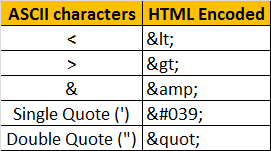
\includegraphics[scale=0.75]{htmlKodiranje.png}
\caption{Output encoding}
\end{center}
\label{kodiranje}
\end{figure}

Rezultat ovoga je prikaz bezobasne renderovane HTML stranice(premda je problem samo preme\v{s}ten sa bezbednosnog na vizuelni).
\subsection{SQL injekcija}
\textbf{SQL injekcija} predstavlja jo\v{s} jedan vid napada injektovanjem kodova(ta\v{c}nije upita) u sajt, ali ovaj put, glavna meta je baza podataka koju koristi server.\\
\textbf{Problem:} Podaci se \v{s}alju od strane korisnika, a sistem ne zna kako da rukuje sa njima.\\
\textbf{Posledice:} 
\begin{enumerate}
	\item neovla\v{s}\'{c}en pristup bazi i njen pregled
	\item modifikovanje baze izvr\v{s}avanjem upita(brisanje podataka, menjanje...)
\end{enumerate}
\subsubsection{SQL injekcija-primena}
Umetanje sql upita, na \v{c}emu se zasniva ovaj metod, naj\v{c}e\v{s}\'{c}e se de\v{s}ava u delu za \textit{Log in}. Razmotrimo slede\'{c}i primer:\\
Predpostavimo da imamo stranicu, koja nakon uspe\v{s}nog prijavljivanja ispisuje informacije o korisniku(njegovo korisni\v{c}ko ime i lozinku, neke informacije o njemu itd.). Prilikom korisni\v{c}kog prijavljivanja, u pozadini se izvr\v{s}ava upit(u op\v{s}tem slu\v{c}aju): \\\textit{SELECT * FROM baza WHERE username='IME' AND password='LOZINKA'}\\
Uneto ime i lozinka predstavljaju parametre za izvr\v{s}avanje ovog upita.\\
Ako bismo u polje za korisni\v{c}ko ime uneli slede\'{c}e:\\
\textit{korisni\v{c}ko ime:} hi' OR '1'='1\\
\textit{lozinka:} hi' OR '1'='1\\
Upit bi izgledao sada ovako:\\
\textit{SELECT * FROM baza WHERE username='hi' OR '1'='1' AND password='hi' OR '1'='1'}\\
Primetimo je izraz 1=1 uvek ta\v{c}an pa je deo za korisni\v{c}ko ime i lozinku krajnje irelevantan.\\
Sistem \'{c}e prijaviti korisnika(naj\v{c}es\'{c}e) sa kredencijalima korisnika koji se nalazi na prvom mestu spiska korisnika iz baze.\\
Naravno, ovo je i dalje upro\v{s}\'{c}en primer, ali svi komplikovaniji se zasnivaju na istoj ideji.
\subsubsection{SQL injekcija-prevencija}
Solucija koja se name\'{c}e za SQL injekciju, jeste da sistem pravilno proverava stringove koji su uneti kao korisni\v{c}ko ime ili lozinka(konkretno u na\v{s}em primeru). Glavni problem i jeste u kori\v{s}\'{c}enju specijalnih karaktera kao \v{s}to su ' = ' ili ' ' ' itd. i sistem mo\v{z}e jednostavno da ih igori\v{s}e.\\
Takodje postoje i sofveri namenjeni proveri 'ranjivosti' sajta injekciji uz predloge dodatne za\v{s}tite.
\subsection{Kontrola pristupa}
Kontrola pristupa predstavlja filtriranje onoga \v{s}ta korisnik mo\v{z}e da vidi ili sa kojim podacima mo\v{z}e da radi,  u zavisnosti od toga koja prava poseduje. Cilj hakera je pristupanje, menjanje ne\v{c}ega za \v{s}ta ne poseduju prava.\\
\textbf{Problem:} Razvijaoci predpostavljaju da, ako ne\v{s}to nije vidljivo korisniku, on ne mo\v{z}e da mu pristupi.\\
\textbf{Posledica:} Neovla\v{s}\'{c}en pristup podacima ili funkcionalnostima.
\subsubsection{Kontrola pristupa-primena}
\textbf{Direct Object References} predstavlja osnovni na\v{c}in zloupotrebe prava pristupa i svodi se na direktno menjanje parametara url-a.\\
Razmotrimo slede\'{c}i primer:\\
Predpostavimo da imamo sajt banke kod koje imamo otvoren ra\v{c}un i nalog na tom sajtu. Nakon uspe\v{s}nog prijavljivanja, url u na\v{s}em pretra\v{z}iva\v{c}u \'{c}e da izgleda ovako:\\
\begin{lstlisting}
http://bank.com/showacc?id=123
\end{lstlisting}
Gde je 123 na\v{s}a reprezentacija sajtu banke. Jednostavnom izmenom '123' na npr. '124' mo\v{z}emo dobiti pregled drugog korisni\v{c}kog naloga(najopasnija promena bi bila sa '123' na '1' jer je to naj\v{c}e\v{s}\'{c}e id admina sa svim pravima pristupa).

Drugi primer, osim pregledanja tudjeg naloga, jeste kori\v{s}\'{c}enje funkcionalnosti za koja nemamo prava.

Predpostavimo da imamo jo\v{s} i dugme za izmenu profila. Klikom na njega, url \'{c}e izgledati ovako:\\
\begin{lstlisting}
http://bank.com/showacc?id=123&action=editProfile
\end{lstlisting}

Predpostavimo da ne mo\v{z}emo mi direktno da izbri\v{s}emo nalog sa sajta banke(nemamo vidljivo dugme za tu funkcionalnost, ve\'{c} moramo da \v{s}aljemo zahtev adminu da to uradi), mo\v{z}emo da predpostavimo(nagadjamo) da i ostale akcije imaju sli\v{c}ne nazive(npr. action=deleteProfile) i da im na taj na\v{c}in neovra\v{s}\'{c}eno pristupimo.\\

Kombinacija prethodna dva pristupa su posledica neovla\v{s}\'{c}enih neograni\v{c}enih prava.
\subsubsection{Kontrola pristupa-prevencija}
Klju\v{c}na stvar jeste da se provere pristupa(autorizacija) rade na serveru(izbegavati ,,Bezbednost prema vidljivosti"Security through obscurity VIKIPEDIJA). 

Naivni pristup bi bio i da se ta provera de\v{s}ava pri svakoj akciji koju korisnik \v{z}eli da izvr\v{s}i(potvrda korisni\v{c}kog imena i lozinke za tu akciju i na osnovu toga provera da li korisnik ima prava za tu akciju).
\section{Zaključak}

\addcontentsline{toc}{section}{Literatura}
\appendix
\bibliography{seminarski}
\bibliographystyle{plain}




\end{document}